\documentclass[Rapport/Rapport_main.tex]{subfiles}
\begin{document}
\section{Metode og proces}
I dette afsnit beskrives processen af et 3. semester projekt, hvor der udvikles et interaktivt Beer Pong bord. Derfor er dette afsnit en opsummering af bilaget \textbf{Proces}. Udover processen vil der også være en beskrivelse af de metoder og redskaber, der er blevet anvendt under forløbet. \\
Der findes følgende to krav omkring processen i 3. semester projektet\cite{Universitet2018}:
\begin{itemize}
    \item ''Anvendelsen af processer og metoder kendt fra projektet på 2. semester, men anvendt iterativt over alle faser.''
    \item ''Iterativ arbejdsmetode, SCRUM, orienteret mod at udvikle nye produkter baseret på HW og SW.''
\end{itemize}
Det er helt tydeligt, at dette projekt skal udvikles iterativt gennem Scrum, og derfor vil det næste underafsnit fokusere på det.

\subsection{Anvendelse af Scrum i PRJ3, Gruppe 7}
Som sagt er dette afsnit dedikeret til at beskrive Scrum anvendelsen for PRJ3 Gruppe 7. Gennem processen er der blevet gjort mange forskellige erfaringer i forhold til, hvad der har fungeret for gruppen. Til at starte med er der udarbejdet en overordnet skitse, der efterfølgende suppleres med forklaringer. Skitsen kan ses i figur \ref{fig:rap_scrum_usage}.
\begin{figure}[H]
    \centering
    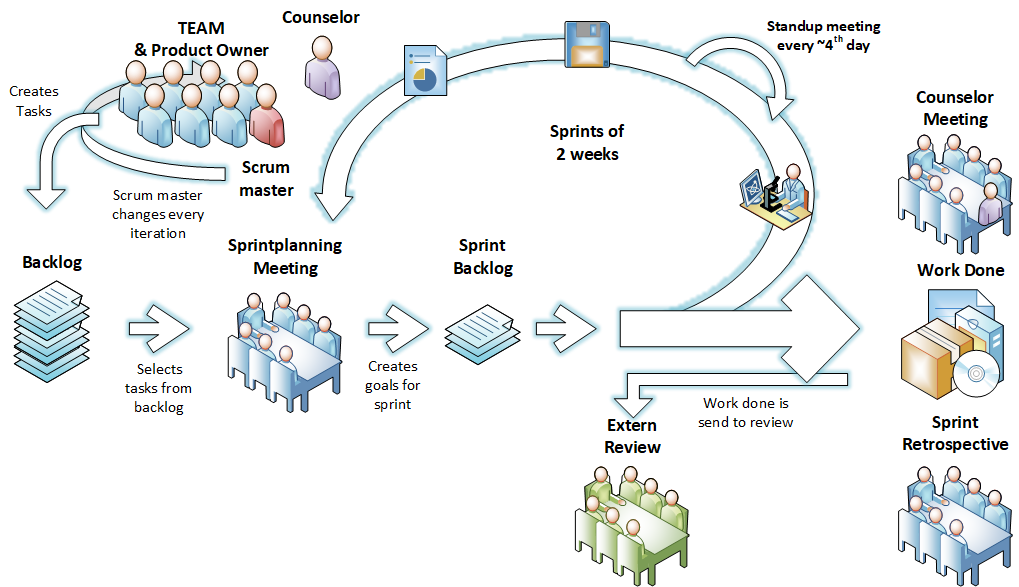
\includegraphics[width=\textwidth]{Processdokument/graphics/Scrum_usage.png}
    \caption{Skitse for hvordan der er anvendt SCRUM i PRJ3 Gruppe 7}
    \label{fig:rap_scrum_usage}
\end{figure}
Af figur \ref{fig:rap_scrum_usage} ses det \textbf{øverst i venstre hjørne}, hvordan gruppen selv har varetaget rollen som Product Owner. Da projektet er specificeret af gruppen, så bestemmer de hvilke funktioner og egenskaber, der prioriteres. Samme sted ses det også, hvordan rollen som Scrum Master er gået på tur efter hvert sprint. Det er gjort for at alle føler ansvaret og erfaringerne, der følger med rollen.\\
\textbf{I midten i venstre side} ses det, hvordan der til Sprint-planlægningsmøder udvælges de relevante tasks fra backloggen, der skal med i det nye sprint. Dette resulterer i en sprint backlog,  der specificerer mål og demoer, der skal fremlægges i slutningen af sprintet.\\
Efter at sprintet er planlagt, kan det ses \textbf{i midten}, at der udføres et sprint med en varighed af 2 uger, hvor der undervejs i sprintet laves Standup Meetings på de aftalte dage. Til disse møder opdateres hele teamet i forhold til, hvor langt man er med opgaver, og om der er problemer, eller mangler hjælp et sted.\\
Til slut i sprintet, ses det \textbf{i højre side}, at der så laves et møde med vejleder. Her evalueres risici i forbindelse med projektet og ud fra disse kan der planlægges tasks. Desuden stilles der forskellige spørgsmål i forbindelse med usikkerheder eller problemer i projektet.  Til sidst laves et retrospektiv på sprintet, hvor der nedskrives positive og negative ting fra det pågældende sprint. Der opsættes så to-tre af de negative punkter, der fokuseres på at forbedre i det næste sprint. Aktionspunkterne fra forrige Sprint tages op for at sikre forbedringer. Undervejs i projektet sendes færdigt materiale til et eksternt review.\\

Til at gøre Scrum nemmere at facilitere, er der blevet anvendt Redmine som værktøj. Grundene til valget er udspecificeret i \textbf{Proces} bilaget i afsnit \fullref{proces:sec:scrum_tools}\\
Hvis der er interesse for anvendelsen af Scrum, samt de erfaringer, der er gjort i løbet af sprintet, så henvises der til afsnit \fullref{proces:sec:experiences_w_scrum} i Proces-dokumentet.

\subsection{Iterativ ASE-udviklingsmodel og SYSML}
Det er et krav for 3. semesterprojektet, at der anvendes metoder og processer, som blev anvendt til 2. semester projektet. På 2. semester blev der til udvikling anvendt ASE-udviklingsmodellen. I dette semester anvendes modellen iterativt og kan ses på figur \ref{fig:rap_ase_model}.
\begin{figure}[H]
    \centering
    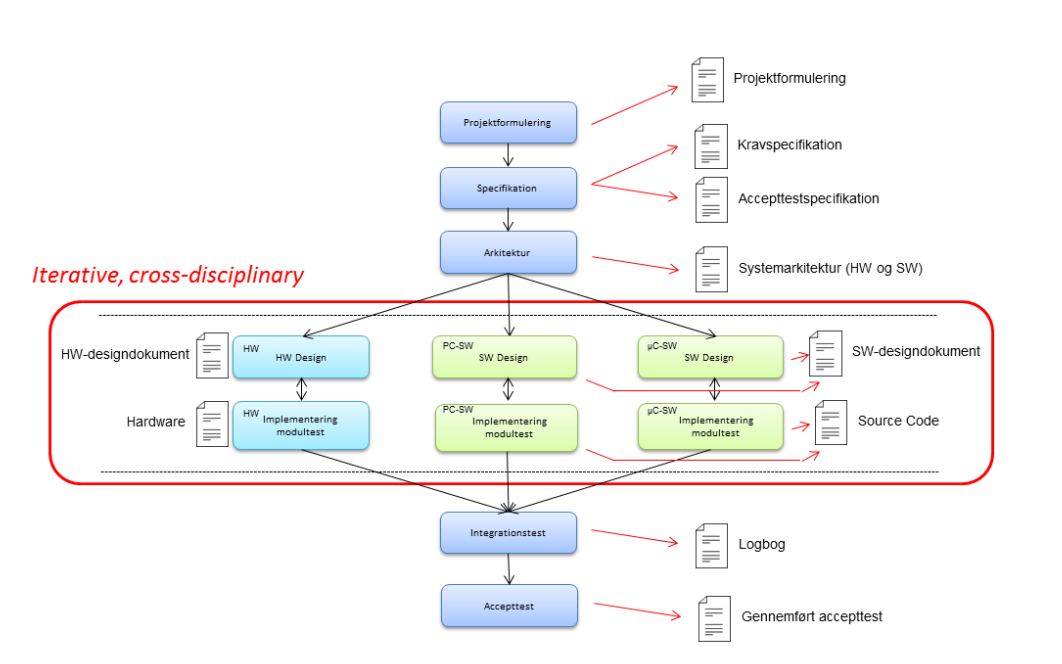
\includegraphics[width=\textwidth]{Processdokument/graphics/ASE_model.png}
    \caption{Udviklingsmodel fra ASE\cite{vejledning_prj3}, der anvendes iterativt over både hardware, software og dokumentation}
    \label{fig:rap_ase_model}
\end{figure}
Derudover anvendes SysML, som redskab til at modellere og beskrive systemet. I SysML anvendes de begreber og metoder, der er stiftet bekendtskab med i 2. semester kurset Indledende System Engineering (ISE). Metoderne kan ses i figur \ref{fig:rap_sysml_usage}.
\begin{figure}[H]
    \centering
    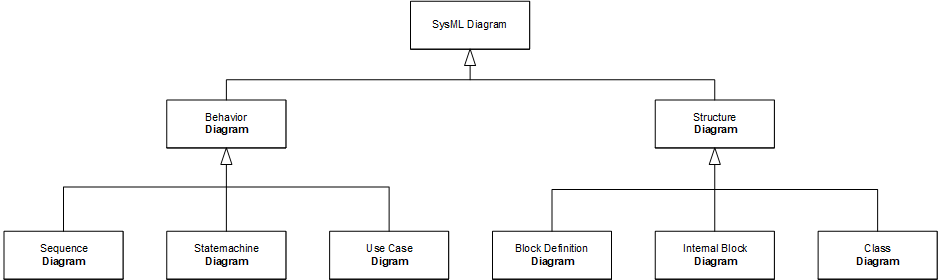
\includegraphics[width=\textwidth]{Processdokument/graphics/Sysml_usage.png}
    \caption{Udarbejdet diagram over de anvendte SysML i Gruppe 7. Systemet beskrives gennem Sekvens-, Statemachine- og Use Case-diagrammer. Strukturen af systemet beskrives ved Block Definition-, Internal Block-diagram og softwarestrukturen gennem Klasse-diagrammer. }
    \label{fig:rap_sysml_usage}
\end{figure}
Den fulde beskrivelse af disse metoder kan ses i \textbf{Proces} bilaget i afsnit \fullref{proces:sec:second_semester_tools}.\\

Udviklingen er nu specifieret, hvilket gør det muligt at påbegynde processen. Som det første analyseres et system ud fra de givne krav. 

\end{document}